%\pagestyle{empty}
\vspace{18cm}
\thispagestyle{plain}
\begin{center}
\textbf{\Huge Capítulo 1}
\end{center}
\begin{center}
\textbf{\Huge Introdução ao Estudo}
\end{center}
\noindent\makebox[\linewidth]{\rule{\textwidth}{1pt}} 
\begin{flushleft}
O Capítulo \ref{chapter:cap1-introducao} tem como objetio apresentar uma Introdução sobre o estudo, apresentando sua motivação, as questões motivadoras da pesquisa, a justifia para o estudo, seus objetivos e qual a hipótese para desenvolvimento da tese.

\end{flushleft}
\noindent\makebox[\linewidth]{\rule{\textwidth}{1pt}} 

Este capítulo se encaixa nas etapas metodológicas a seguir:
\begin{figure}[ht]
\centering
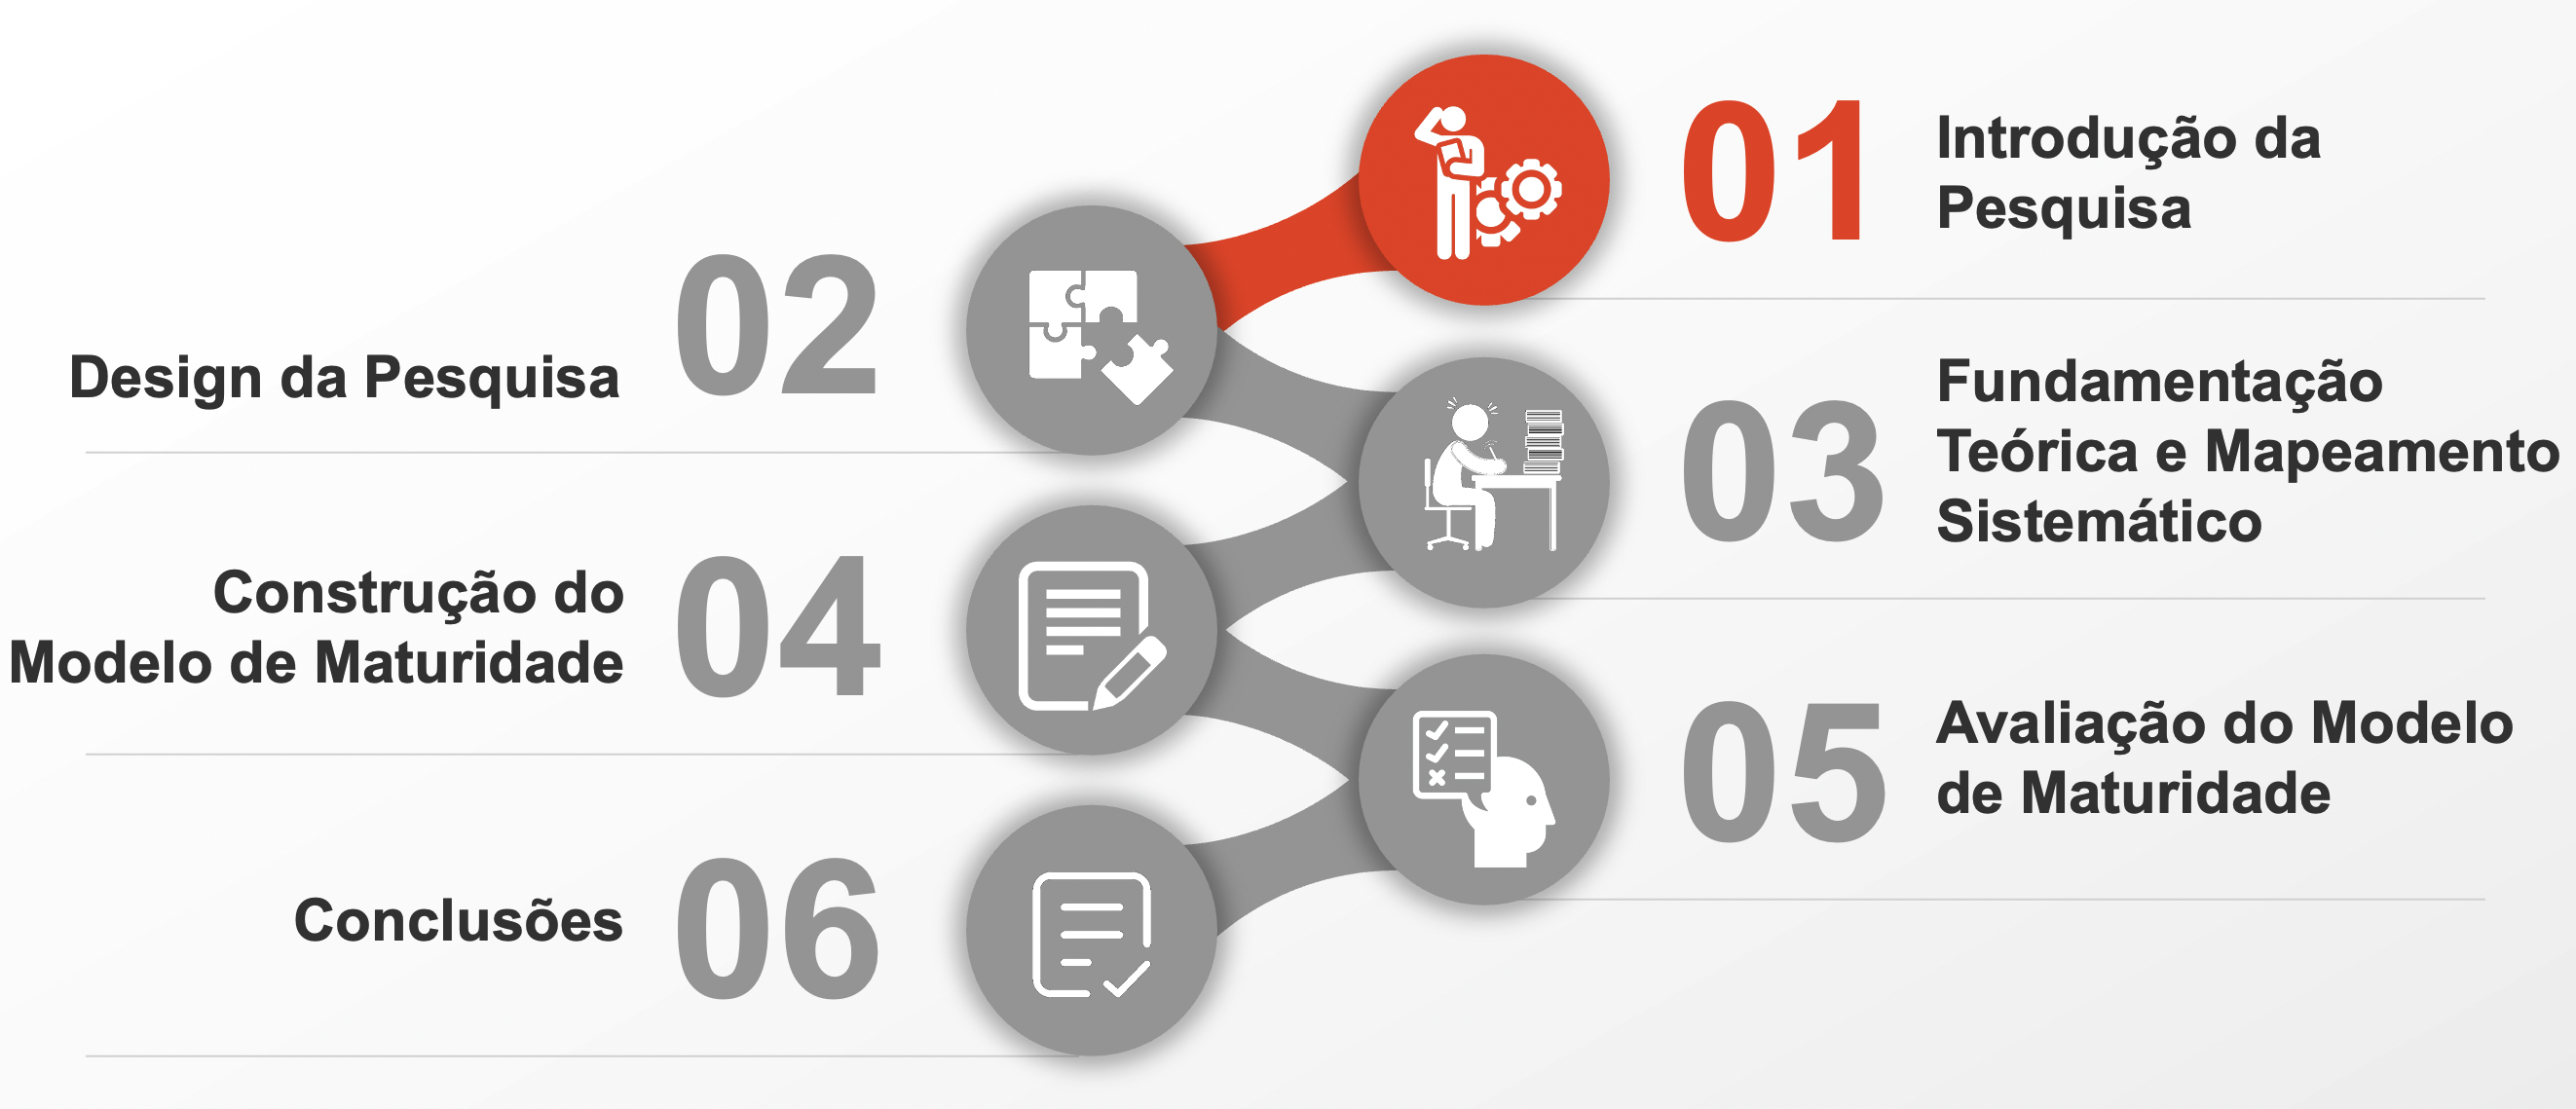
\includegraphics[width=15cm]{images/part-capitulo1.png}
\label{fig:metodologia-cap1}
\end{figure}